%==============================================================================
%  The Journal of Finance and Data Science -- Research article (elsarticle)
%  Anonymized manuscript for double-anonymized review: no author details.
%  Compile with pdfLaTeX, three runs. The bibliography is inline (no BibTeX).
%==============================================================================
\documentclass[preprint,12pt,authoryear,a4paper]{elsarticle}

\usepackage[T1]{fontenc}
\usepackage[utf8]{inputenc}
\usepackage{lmodern}
\usepackage{amsmath}
\usepackage{amssymb}
\usepackage{array}
\usepackage{booktabs}
\usepackage{multirow}
\usepackage{longtable}
\usepackage{graphicx}
\usepackage{xcolor}
\usepackage{float}
\usepackage{algorithm}
\usepackage{algpseudocode}
\usepackage{tikz}
\usepackage{pgfplots}
\pgfplotsset{compat=1.17}
\usetikzlibrary{positioning,arrows.meta,calc,fit,backgrounds}
\usepackage{microtype}
\usepackage{xurl}
\usepackage[hidelinks]{hyperref}
\setlength{\emergencystretch}{3em}
\newcolumntype{L}[1]{>{\raggedright\arraybackslash}p{#1}}
\renewcommand{\topfraction}{0.9}
\renewcommand{\bottomfraction}{0.8}
\renewcommand{\textfraction}{0.07}
\renewcommand{\floatpagefraction}{0.75}
\setcounter{topnumber}{3}
\setcounter{bottomnumber}{2}
\setcounter{totalnumber}{4}

%---- colours and node styles ---------------------------------------------------
\definecolor{cInput}{HTML}{455A64}\definecolor{cData}{HTML}{1565C0}
\definecolor{cPrice}{HTML}{E65100}\definecolor{cEval}{HTML}{6A1B9A}
\definecolor{cGood}{HTML}{2E7D32}\definecolor{cBad}{HTML}{C62828}
\definecolor{cWarn}{HTML}{AD1457}
\tikzset{
  base/.style={rounded corners=2pt,draw,align=center,font=\small,minimum height=8mm,inner sep=4pt,line width=0.5pt},
  io/.style={base,fill=cInput!12,draw=cInput}, dnode/.style={base,fill=cData!12,draw=cData},
  pnode/.style={base,fill=cPrice!14,draw=cPrice}, enode/.style={base,fill=cEval!12,draw=cEval},
  gnode/.style={base,fill=cGood!12,draw=cGood}, bnode/.style={base,fill=cBad!12,draw=cBad},
  wnode/.style={base,fill=cWarn!12,draw=cWarn},
  layer/.style={text width=3.3cm,minimum height=3.0cm,anchor=center,font=\footnotesize},
  arr/.style={-{Latex[length=2.2mm]},line width=0.7pt},
  darr/.style={-{Latex[length=2.2mm]},line width=0.7pt,dashed},
  lbl/.style={font=\scriptsize\itshape,fill=white,inner sep=1pt}}

\journal{The Journal of Finance and Data Science}

\begin{document}

\begin{frontmatter}

\title{Beyond Directional Accuracy: A Verified Walk-Forward Framework for
Machine-Learning Cryptocurrency Trading}

\begin{abstract}
Most studies judge machine-learning forecasts of cryptocurrency returns by
directional accuracy alone. Accuracy does not show whether a model adds anything to
a simple rule, or whether it still earns money after trading costs. We build an
evaluation framework that links forecasting, statistical testing and trading
economics, avoids look-ahead leakage and tests its own code, and we apply it to
daily Binance spot data for Bitcoin, Ether and Dogecoin. The framework uses 30
causal features, walk-forward validation with in-fold scaling and a training--test
gap, paired tests against simple baselines, measures based on the size of price
moves, and a break-even cost estimated together with turnover. Its tests caught all
eight rule violations that we put back into the backtest engine. Over 5,562
out-of-sample forecasts from July 2020 to March 2026, a regularized logistic model
is correct 52.95\% of the time (95\% interval 51.45--54.41\%) and beats a coin flip
on every asset. A one-day reversal rule scores 52.88\%, so much of this skill is
shared with it, but the model is better on large moves. It has the higher
return-weighted hit rate on all three assets, and its long/short book earns a gross
Sharpe ratio of 0.54, against 0.004 for the reversal rule. At 9 basis points per
unit of turnover the net Sharpe ratio is 0.11 and the break-even cost is 11.4 basis
points, while a long-or-cash version reaches 0.71. The bootstrap intervals are
still wide. The full analysis is reproduced by one command.
\end{abstract}

\begin{highlights}
\item A tested walk-forward framework for daily crypto forecasting without leakage
\item Logistic forecasts beat a coin flip on BTC, ETH and DOGE (52.95\% pooled)
\item Size-aware tests show where the model is better than a one-day reversal rule
\item A joint return and turnover bootstrap puts the break-even cost at 11.4 bps
\item Mutation tests confirm the engine's safeguards: 8 of 8 violations caught
\end{highlights}

\begin{keyword}
Financial machine learning \sep Walk-forward validation \sep Cryptocurrency
\sep Forecast evaluation \sep Transaction costs \sep Backtest verification
\JEL G17 \sep C53 \sep C58 \sep G14
\end{keyword}

\end{frontmatter}

%==============================================================================
\section{Introduction}\label{sec:intro}
%==============================================================================

Machine-learning models are now a common tool for forecasting cryptocurrency
prices. Most studies report their success as directional accuracy, which is the
share of days on which the next move is predicted correctly. Accuracy is easy to
compute and easy to compare, but it leaves three practical questions open. Does the
model know anything that a simple rule does not know? Does it get the right days
correct, that is, the days with large moves that decide most of the profit and
loss? And does its edge survive the cost of trading on it? A good model alone cannot
answer these questions. We also need an evaluation process in which forecasting,
testing and trading economics are linked, and in which the code behind each number
can be trusted.

In this paper we build such a process and apply it to daily Binance spot data for
Bitcoin (BTC), Ether (ETH) and Dogecoin (DOGE) from 2017 to 2026. The framework has
five layers and a verification layer under them (Figure~\ref{fig:framework}). The
data layer checks the input files and records their hashes. The feature layer
builds 30 strictly causal predictors, and it screens any feature that is supposed
to come from outside the market for hidden dependence on prices. The learning layer
fits the models in an expanding walk-forward design. Preprocessing is fitted inside
each fold, and there is a gap between the training data and the test data. The
inference layer compares every model with simple baselines on the same dates. It
uses paired tests that allow for dependence, a bootstrap that resamples dates, and
measures that take the size of moves into account. The economic layer turns the
forecasts into a portfolio, estimates the break-even trading cost together with
turnover, and checks the result against a separate cash ledger. The verification
layer writes the timing and accounting rules of the backtest engine as executable
contracts, and it uses mutation testing to confirm that the tests really catch
violations.

We apply the framework to $5{,}562$ out-of-sample forecasts made between July 2020
and March 2026, and we find four main results. First, an $\ell_2$-regularized
logistic regression is correct $52.95\%$ of the time. The date-synchronized $95\%$
interval for this pooled accuracy is $51.45$--$54.41\%$, and the model beats a coin
flip on every asset. The Pesaran--Timmermann test confirms that its calls are
related to the realized direction ($p$-values from $0.008$ to $0.016$), and the
model is more accurate than gradient-boosted trees on all three assets. Second, the
comparison with baselines shows that much of this skill is shared with one-day
reversal. A rule that simply bets against the previous day's move is correct
$52.88\%$ of the time, and the model agrees with it on $71\%$ of asset-days. Third,
the model is different from that rule in magnitude. On the days where the two
disagree, the model tends to be the one that gets the large moves right. It has the
higher return-weighted hit rate on all three assets, and an equal-weight long/short
book built on its forecasts earns a gross Sharpe ratio of $0.54$, against $0.004$
for the same book built on the reversal rule. Fourth, the economic result is
positive at realistic costs. At 9 basis points (bps) per unit of turnover the net
Sharpe ratio is $0.11$, the estimated break-even cost is $11.4$ bps, and a
long-or-cash version reaches $0.71$. With less than six years of daily data the
bootstrap intervals around these numbers are wide, and we report them everywhere.

Two more results are about the framework itself. Its provenance screen flags a
synthetic sentiment series as price-derived on all three assets. This series was
built from daily prices as a placeholder during development, and on one of the
assets a linear check would have missed it. The verification layer catches all eight
contract violations that we put back into the engine. The full pipeline runs again
from one command, and in a clean environment with the pinned library versions it
gives the same primary output files byte for byte.

The paper makes five contributions.
\begin{enumerate}
\item \textbf{An end-to-end evaluation algorithm} (Algorithm~\ref{alg:framework}).
It links forecasting, testing and trading economics, stores the date of every
forecast, saves every fitted pipeline and produces every reported number from one
command.
\item \textbf{A leakage-safe design}. Features are causal and are checked by a
prefix-invariance test, preprocessing is fitted inside each fold, training and test
data are separated by a gap, and a rank-based provenance screen checks external
features.
\item \textbf{Inference that uses baselines and magnitude}. We use paired HAC
comparisons against simple rules with no parameters, a bootstrap that resamples
dates for pooled statistics, and return-weighted measures that show where the value
of a model comes from.
\item \textbf{Cost-aware economics}. We estimate a break-even cost together with
turnover, and we report a full cost curve, policy variants and a cash ledger that
is reconciled separately.
\item \textbf{A verified implementation}. Ten executable contracts cover timing,
accounting, statistics and estimation, and eight of them are confirmed by mutation
testing.
\end{enumerate}

We use simple, well-known models on purpose. Our aim is a process that tells a
researcher what a model adds and whether it can pay for its trading costs. Any
classifier can be used in the learning layer.

%==============================================================================
\section{Related work}\label{sec:related}
%==============================================================================

\subsection{Backtest overfitting and data snooping}

Most work on the reliability of backtests is about inference, that is, how much an
attractive result should be discounted for the number of alternatives that were
tried. \citet{white2000reality} proposed the Reality Check bootstrap.
\citet{sullivan1999data} applied it to thousands of technical trading rules on a
century of Dow Jones data, and they showed that the apparent significance of the
best rule depends strongly on taking the whole set of searched rules into account.
\citet{hansen2005test} improved the procedure into a test for superior predictive
ability. \citet{bailey2014deflated} deflate the Sharpe ratio for selection and
non-normality. \citet{harvey2016cross} argue that the usual $t>2$ hurdle is far too
low, given how many factors have been tested, and \citet{hou2020replicating} find
that most of several hundred published anomalies do not replicate under consistent
methods. \citet{lopezdeprado2018advances} gives the purging and embargo tools that
we build on, and \citet{arnott2019backtesting} set out a protocol for
machine-learning backtests.

These studies usually take the backtest engine as given and ask what can be
concluded from its output. Our framework adds a layer below this, in which the
engine itself is checked. Errors in backtest code tend to have large effects, not
small ones, and a natural tool for finding them is mutation testing. Mutation
testing is standard in software engineering \citep{jia2011analysis}, but as far as
we know it is rarely reported in empirical finance.

\subsection{Benchmarks and tests of directional forecasts}

\citet{makridakis2018statistical} show that complex forecasting methods often do
not beat simple statistical benchmarks, and that this comparison is often not made
at all. \citet{pesaran1992simple} test whether predicted and realized directions
are independent. This is the hypothesis that a directional forecast really has to
reject, because a hit rate above one half is not enough when up days and down days
are not equally common. \citet{diebold1995comparing} compare two forecasts through
their loss differences on the same observations, and \citet{newey1987simple} give
the autocorrelation-consistent variance that we use for these differences. For
pooled statistics, Sharpe ratios and costs we use the stationary bootstrap of
\citet{politis1994stationary}, and we resample dates rather than asset-days. For
per-asset hit rates we use the score interval of \citet{wilson1927probable}.

\subsection{Short-horizon predictability in cryptocurrency returns}

Short-horizon reversal is well documented in equities
\citep{jegadeesh1990evidence,lo1990contrarian}. In cryptocurrency markets,
\citet{caporale2019reverse} find unusually large price moves on the day after an
overreaction, but no strategy that profits from them, and \citet{liu2021risks} find
time-series momentum at weekly horizons. Machine-learning studies of cryptocurrency
direction report results that depend on the horizon, the inputs and the
specification. \citet{jaquart2021short}, in this journal, compare several model
families at horizons of one to sixty minutes. A long--short strategy based on their
forecasts earns high returns before transaction costs and negative returns after
them. \citet{gradojevic2023forecasting} use technical indicators at hourly and daily
frequencies and find that forecasting performance depends on the horizon and the
specification. For equities, \citet{gu2020empirical} find large gains from trees
and neural networks, which they link to nonlinear interactions among many
predictors. With a small single-asset feature set we find the opposite ranking:
logistic regression is more accurate than boosted trees on all three assets.
\citet{fama1970efficient} and \citet{timmermann2004efficient} give the prior that
we start from. Predictability may exist, but it should be small, unstable and
limited by trading costs.

\subsection{Leakage}

\citet{kaufman2012leakage} define leakage as the use of information that would not
be available at prediction time. They stress that a variable must be judged against
the timing of the prediction task and not by its name. \citet{bergmeir2012use} and
\citet{cerqueira2020evaluating} study when cross-validation is valid for time
series. The provenance screen in Section~\ref{ssec:provenance} deals with a case
that is inside these definitions but outside the usual checks, namely a feature
whose name suggests an external source but whose values are computed from the
prices themselves.

%==============================================================================
\section{The proposed framework}\label{sec:framework}
%==============================================================================

\subsection{Overview}

Figure~\ref{fig:framework} gives a summary of the framework and
Algorithm~\ref{alg:framework} lists its steps. Two design principles are used in
every layer. The first is strict information timing. Nothing that becomes known
only after the close of day $t$ may enter a forecast made at that close, and every
forecast is stored with its decision date, label date and fold. The second is
independent verification. Every important quantity is either computed twice, along
different code paths, or checked against a fixture with a known answer.
Section~\ref{sec:method} gives the statistical and economic details. This section
describes the parts of the framework that protect the computation itself.

\begin{figure}[htbp]\centering
\resizebox{\textwidth}{!}{%
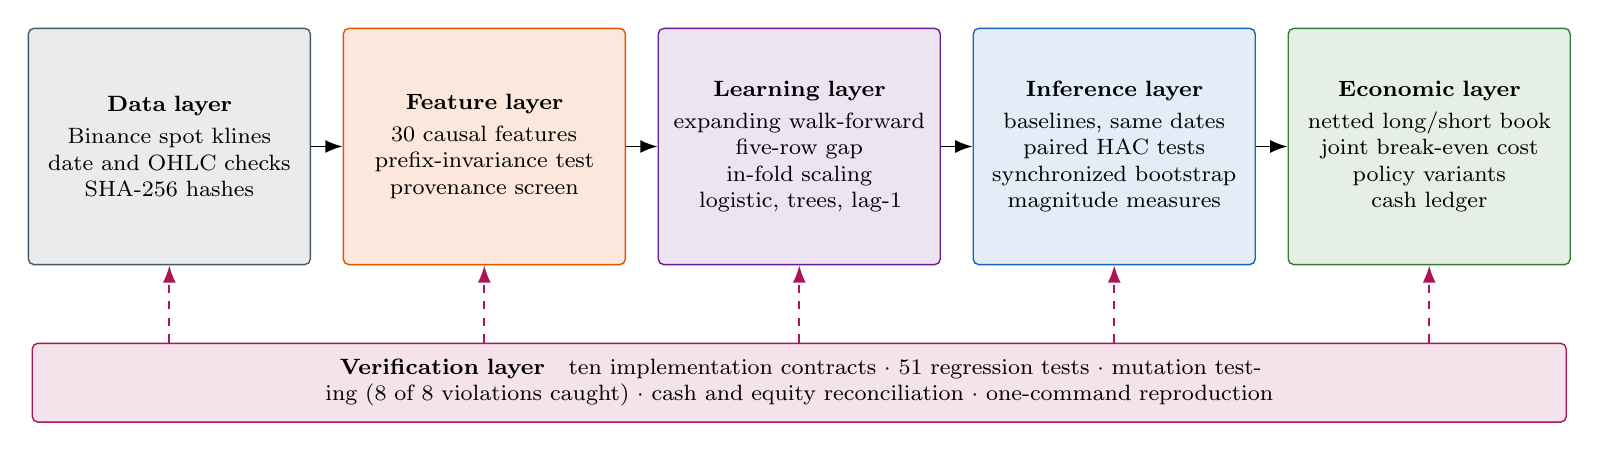
\begin{tikzpicture}[x=1cm,y=1cm]
\node[io, layer]    (L1) at (0,0)    {\textbf{Data layer}\\[2pt] Binance spot klines\\ date and OHLC checks\\ SHA-256 hashes};
\node[pnode, layer] (L2) at (4,0)    {\textbf{Feature layer}\\[2pt] 30 causal features\\ prefix-invariance test\\ provenance screen};
\node[enode, layer] (L3) at (8,0)    {\textbf{Learning layer}\\[2pt] expanding walk-forward\\ five-row gap\\ in-fold scaling\\ logistic, trees, lag-1};
\node[dnode, layer] (L4) at (12,0)   {\textbf{Inference layer}\\[2pt] baselines, same dates\\ paired HAC tests\\ synchronized bootstrap\\ magnitude measures};
\node[gnode, layer] (L5) at (16,0)   {\textbf{Economic layer}\\[2pt] netted long/short book\\ joint break-even cost\\ policy variants\\ cash ledger};
\draw[arr] (L1.east) -- (L2.west);
\draw[arr] (L2.east) -- (L3.west);
\draw[arr] (L3.east) -- (L4.west);
\draw[arr] (L4.east) -- (L5.west);
\node[wnode, text width=19.2cm, minimum height=1.0cm, font=\footnotesize] (V) at (8,-3.0)
  {\textbf{Verification layer}\quad ten implementation contracts $\cdot$ 51 regression tests $\cdot$ mutation testing (8 of 8 violations caught) $\cdot$ cash and equity reconciliation $\cdot$ one-command reproduction};
\foreach \n in {L1,L2,L3,L4,L5}{\draw[darr, draw=cWarn] (V.north -| \n.south) -- (\n.south);}
\end{tikzpicture}}
\caption{The evaluation framework. Forecasts move from left to right; the
verification layer checks the computations in every layer.}
\label{fig:framework}
\end{figure}

\begin{algorithm}[htbp]
\caption{Verified walk-forward evaluation}
\label{alg:framework}
\begin{algorithmic}[1]
\Require daily bars for assets $j\in\mathcal{J}$; initial window $m=1{,}000$; test
block $b=250$; gap $e=5$; cost $c$; bootstrap replicates $B$ and mean block length $L$
\State Validate dates, prices and OHLC bounds; record the SHA-256 hash of each input
\State Build causal features $x_{j,t}$ and labels $y_{j,t}=\mathbf{1}(C_{j,t+1}>C_{j,t})$; drop warm-up rows
\State Screen each external feature; exclude it if its rank correlation with same-day returns exceeds $\tau$
\For{each asset $j$ and fold $k=0,1,\dots$ with $a_k=m+e+bk<n_j$}
  \State Fit scaler and classifier on rows $i<a_k-e$; save the fitted pipeline
  \State Forecast rows $a_k\le i<\min(a_k+b,\,n_j)$; record all baseline forecasts on the same dates
\EndFor
\State Per asset: Wilson intervals, Pesaran--Timmermann tests, paired HAC differences against inverse persistence
\State Pooled: date-synchronized stationary bootstrap with $B$ replicates and mean block length $L$
\State Magnitude: return-weighted hit rates and accuracy by size of the next-day move
\State Portfolio: $w_{j,t}=s_{j,t}/J_t$; gross return $g$, turnover $q$, net return $g-cq$; Sharpe ratios and $c^{*}=\bar g/\bar q$ with joint bootstrap intervals
\State Cash ledger: book every leg with its own fee; assert agreement with the closed-form return
\State Verification: run the regression tests; re-insert each contract violation and require the named test to fail
\Ensure dated forecasts, fitted pipelines, inference tables, cost curve and verification report
\end{algorithmic}
\end{algorithm}

\subsection{Implementation contracts}\label{ssec:contracts}

Errors in backtest code are easy to miss, because a faulty engine still produces
numbers that look reasonable. For this reason we write the rules of the engine as
ten contracts in four groups, together with two reporting conventions
(Table~\ref{tab:contracts}). Each contract protects against one specific pitfall.
Several of these pitfalls came up while we were building the system, and this is
why we test for them directly. Every contract is enforced by at least one
regression test with a known answer. For eight of them we go one step further and
confirm, by mutation testing, that putting the violation back makes the named test
fail (Section~\ref{sec:verification}).

\begin{table}[htbp]\centering\small
\caption{Implementation contracts of the backtest engine. \emph{Mutation}:
confirmed by re-inserting the violation (Table~\ref{tab:mutation}). \emph{Test}:
enforced by a dedicated regression test. \emph{Definition}: a reporting
convention.}
\label{tab:contracts}
\begin{tabular}{@{}lL{0.40\textwidth}L{0.31\textwidth}l@{}}
\toprule
ID & Contract & Pitfall it prevents & Check \\
\midrule
\multicolumn{4}{@{}l}{\emph{Timing}} \\
C1  & Prices are looked up at or before the signal time & Fills against a bar that has not closed & Mutation \\
C2  & Orders fill at the open of the next bar & Same-bar execution & Test \\
C3  & Stops and targets are checked against each bar's high and low & Missed intrabar exits & Mutation \\
\midrule
\multicolumn{4}{@{}l}{\emph{Accounting}} \\
C4  & Each position is valued against its own asset's prices & Cross-asset pricing & Test \\
C5  & Short positions lose value when their price rises & Inverted short P\&L & Mutation \\
C6  & Fees are charged on each leg's own notional & Cash that disagrees with reported fees & Mutation \\
\midrule
\multicolumn{4}{@{}l}{\emph{Statistics}} \\
C7  & Sharpe ratios use equity-curve returns at the bar frequency & Annualizing per-trade returns & Mutation \\
C8  & Monte Carlo resamples trades with replacement & A simulation whose paths are all identical & Mutation \\
\midrule
\multicolumn{4}{@{}l}{\emph{Estimation sample}} \\
C9  & The scaler is fitted on training rows only and saved with the model & In-sample or single-row scaling & Mutation \\
C10 & Training and test samples are separated by a gap & Overlap between training and test data & Mutation \\
\midrule
\multicolumn{4}{@{}l}{\emph{Reporting conventions}} \\
R1  & Calmar ratio uses the maximum peak-to-trough drawdown & An unrelated denominator & Definition \\
R2  & Accuracy-derived quantities are not labeled as risk or profit measures & Misleading metric names & Definition \\
\bottomrule
\end{tabular}
\end{table}

\paragraph{Timing} Prices are looked up only at or before the signal time (C1).
This is done by a binary search over $\{i: t_i\le t_{\text{signal}}\}$ and not by a
nearest-bar search, which can pick a bar that has not closed yet. Orders fill at the
open of the next bar (C2). Stops and targets are checked against the high and low
of every bar (C3). When one bar touches both, we assume that the stop fills first,
because daily OHLC data cannot show the order.

\paragraph{Accounting} Each position is valued with the prices of its own asset
(C4), and the portfolio value is
\begin{equation}
V_t=\text{cash}_t+\sum_{j\in\text{long}} q_j\,p^{(j)}_t-\sum_{j\in\text{short}} q_j\,p^{(j)}_t ,
\label{eq:equity}
\end{equation}
so a short position loses value when its price goes up (C5). Fees are charged on the
own notional of each leg (C6), so the cash that is charged always equals the
reported fees.

\paragraph{Statistics} Sharpe ratios are computed from equity-curve returns that
are sampled at the bar frequency (C7),
\begin{equation}
S=\frac{\overline{r-r_f}}{\operatorname{sd}(r-r_f)}\sqrt{P},
\qquad
P=\frac{\text{seconds per year}}{\operatorname{median}\{t_{i+1}-t_i\}},
\label{eq:sharpe}
\end{equation}
and not by annualizing per-trade returns with a fixed factor such as $\sqrt{252}$,
which is undefined when trades do not arrive on a fixed clock. All research results
in this paper set $r_f=0$. Monte Carlo analysis resamples trades with replacement
and tracks drawdown (C8). Simply permuting and summing trade profits would give the
same total on every path.

\paragraph{Estimation sample} The feature scaler is fitted on training rows only
and is saved with the model (C9). If it were fitted at inference time on a single
row, it would map every feature to zero. Training and test samples are separated by
a gap (C10),
\begin{equation}
\mathcal{T}_{\text{train}}=[0,k),\qquad
\mathcal{T}_{\text{test}}=[k+e,n),\qquad
e\ge L_{\text{seq}}+h,
\label{eq:embargo}
\end{equation}
where $L_{\text{seq}}$ is the length of any sequence window and $h$ is the label
horizon \citep{lopezdeprado2018advances}.

\paragraph{Reporting conventions} The Calmar ratio divides the annualized return by
the maximum peak-to-trough drawdown (R1). Quantities derived from accuracy are never
called risk or profit measures (R2). For accuracy $a$, a ``Sharpe ratio'' built by
scoring correct calls as $+1$ and wrong calls as $-1$ equals
$(2a-1)/\bigl(2\sqrt{a(1-a)}\bigr)$, so it carries no information beyond $a$. These
two conventions are definitions and not computations, so we state them without
separate tests.

\paragraph{Independent checks} When two metrics are produced along different code
paths, errors in backtest code can hide each other. For example, a sign error in the
valuation of short positions corrupts the equity curve, but it never reaches a
Sharpe ratio that is computed from the trade list. So the framework reconciles each
economic quantity with an independent calculation: the equity curve with the summed
trade profits, the cash ledger with a closed-form return formula, and the saved
models with the stored forecasts.

\subsection{Provenance screening}\label{ssec:provenance}

Some features come with names that promise information from outside the market,
such as news sentiment. Before such a feature can enter a model, the framework
checks how well it can be rebuilt from prices of the same day. We show the screen on
a synthetic sentiment series that was generated from daily prices as a placeholder
during development, because free news archives usually go back only about 30 days.
For each daily bar, the generator computes the open-to-close return
$u_t=(C_t-O_t)/O_t$ and sets
\begin{equation}
s_t=\operatorname{round}_3\Bigl[\operatorname{clip}\bigl(\operatorname{clip}(15u_t,-1,1)+\epsilon_t,\,-1,\,1\bigr)\Bigr],
\qquad \epsilon_t\sim\mathcal{U}(-0.2,0.2),
\label{eq:sentgen}
\end{equation}
and then adds a label (positive or negative beyond $\pm0.3$, neutral otherwise) and
a template headline.

\begin{table}[htbp]\centering\small
\caption{Provenance screen for the synthetic sentiment series: dependence on the
same day's open-to-close return and on the next day's close-to-close return. Sign
agreement is the share of days on which the two have the same sign.}
\label{tab:leak}
\begin{tabular}{@{}lrrrrrr@{}}
\toprule
 & & \multicolumn{3}{c}{Same day, $u_t$} & \multicolumn{2}{c}{Next day, $r_{t+1}$} \\
\cmidrule(lr){3-5}\cmidrule(l){6-7}
Asset & Days & Pearson & Rank & Signs agree & Pearson & Signs agree \\
\midrule
BTC  & $3{,}150$ & $0.916$ & $0.945$ & $87.0\%$ & $-0.018$ & $47.2\%$ \\
ETH  & $3{,}150$ & $0.907$ & $0.968$ & $89.2\%$ & $-0.034$ & $46.2\%$ \\
DOGE & $2{,}463$ & $0.519$ & $0.972$ & $90.1\%$ & $-0.015$ & $46.3\%$ \\
\bottomrule
\end{tabular}
\end{table}

Table~\ref{tab:leak} reports the screen. The score has the same sign as the same
day's return on $87$--$90\%$ of days and has rank correlations of $0.95$--$0.97$
with it, while it has almost no relation with the next day's return. So the screen
flags it on every asset, and the framework keeps it out of all models. The choice
of statistic is important here. A linear fit on the same-day return explains $84\%$
of the score's variance for BTC and $82\%$ for ETH, but only $27\%$ for DOGE,
because the large daily moves of DOGE often push $15u_t$ past the clipping bounds. A
linear threshold would therefore have passed the DOGE series, while its rank
correlation of $0.97$ flags it. If such a score is used to explain the same day's
direction, it is the same as using the target as a feature. If it is used after the
close to forecast the next day, it does not leak future information, but it adds
nothing that prices do not already contain.

%==============================================================================
\section{Data and experimental design}\label{sec:method}
%==============================================================================

\subsection{Instrument and data}

We use daily Binance spot klines for BTCUSDT, ETHUSDT and DOGEUSDT, quoted in USDT
\citep{binance2026data}. Each bar covers one UTC calendar day and is fully known
only after 24:00 UTC. The fields are the open, high, low and close prices, base and
quote volume, number of trades and taker-buy base volume. It is important to name
the instrument, because fees, shorting and funding are different for spot, margin
and perpetual futures. The long/short strategies take short positions, which need
margin on the spot market. We treat this as an idealization and come back to it in
Section~\ref{sec:limitations}.

The BTC and ETH files run from 17 August 2017 to 1 April 2026 ($3{,}150$ days each),
and the DOGE file runs from 5 July 2019 to 1 April 2026 ($2{,}463$ days). No date is
missing or repeated, all prices are positive, and every bar satisfies
$L_t\le\min(O_t,C_t)\le\max(O_t,C_t)\le H_t$. As a provenance check, we compared all
eight numeric fields for $275$ asset-days (July 2019, January 2023 and March 2026
for each asset) with the checksum-verified monthly archives of the exchange, and
every field matched to a relative tolerance of $10^{-10}$. This check covers the
sampled months, not the whole history.

\subsection{Sample construction}

\begin{table}[htbp]\centering\small
\caption{Sample reconciliation. Usable rows exclude the 60-day feature warm-up and
the last two days of each file. Out-of-sample (OOS) forecasts start after the
first $1{,}005$ usable rows ($1{,}000$ for initial training plus a five-row gap).
The panel has $5{,}562$ asset-day forecasts on $2{,}083$ distinct decision dates.}
\label{tab:data}
\resizebox{\textwidth}{!}{%
\begin{tabular}{@{}llrrrrl@{}}
\toprule
Asset & Data period & Raw rows & Usable rows & OOS forecasts & Folds & OOS decision dates \\
\midrule
BTCUSDT  & 2017-08-17 to 2026-04-01 & $3{,}150$ & $3{,}088$ & $2{,}083$ & 9 & 2020-07-17 to 2026-03-30 \\
ETHUSDT  & 2017-08-17 to 2026-04-01 & $3{,}150$ & $3{,}088$ & $2{,}083$ & 9 & 2020-07-17 to 2026-03-30 \\
DOGEUSDT & 2019-07-05 to 2026-04-01 & $2{,}463$ & $2{,}401$ & $1{,}396$ & 6 & 2022-06-04 to 2026-03-30 \\
\midrule
Panel    &                          &           &           & $\mathbf{5{,}562}$ & 24 & $2{,}083$ dates \\
\bottomrule
\end{tabular}}
\end{table}

Three sample definitions are used in this paper (Table~\ref{tab:data}). Raw rows
are the rows of the input files. Usable rows drop the first 60 days, which the
longest rolling windows need, and the last two days. The final decision date is 30
March 2026, whose label uses the close of 31 March, and 1 April is an unused buffer
that we keep so that all three assets share one cutoff. Usable rows are therefore
raw rows minus 62. Out-of-sample forecasts begin after the first $1{,}005$ usable
rows. The panel has $5{,}562$ asset-day forecasts but only $2{,}083$ distinct
decision dates: two assets on the 687 dates before DOGE enters (17 July 2020 to 3
June 2022) and three assets on the other $1{,}396$ dates. BTC and ETH move
together, so asset-days are not independent observations, and the inference in
Section~\ref{ssec:inference} resamples dates and not asset-days.

\subsection{Features}

The models use 30 features, and each one is computed from bars dated $t$ or earlier
(\ref{app:features}). They are log returns over 1, 2, 3, 5, 10 and 20 days; rolling
volatility and close-price $z$-scores over 5, 10, 20 and 60 days; three measures of
the shape of the bar; seven trading-activity measures built from the kline fields
(taker-buy share, average trade size, trade count and volume, as $z$-scores or
ratios); and RSI, a MACD histogram, Bollinger-band position, normalized ATR and a
day-of-week encoding. A test checks the number of features, and it also checks that
the features for date $t$ do not change when later rows are deleted. This is a
direct check of causality.

This is a single-asset technical feature set. It does not include the inputs that
are most specific to cryptocurrency markets, such as perpetual funding rates, open
interest, basis, liquidations, order-book imbalance, exchange flows and lead--lag
effects across assets. This makes it a conservative test of what price and activity
data alone can give.

\subsection{Target, validation and models}

The target is $y_t=\mathbf{1}(C_{t+1}>C_t)$. Ties happen on 6 of the $5{,}562$
evaluation asset-days, and they are put in class zero. Validation is an
expanding-window walk-forward (Figure~\ref{fig:wf}). With usable rows indexed
$i=0,\dots,n-1$, fold $k$ tests rows $a_k\le i<\min(a_k+250,n)$, where
$a_k=1{,}005+250k$, and trains on rows $i<a_k-5$. A final block is kept only if it
has at least 30 rows. BTC and ETH have nine folds (eight of 250 days and a last one
of 83), and DOGE has six (five of 250 and one of 146). The five excluded rows
separate the last training label from the first test forecast. For example, in the
first BTC fold the last training label is the close of 12 July 2020, and the first
test forecast is made at the close of 17 July. Rolling features in a test fold do
share past bars with the training data, but shared history is not future
information. Every forecast is made only once, out of sample.

\begin{figure}[htbp]\centering
\resizebox{0.95\textwidth}{!}{%
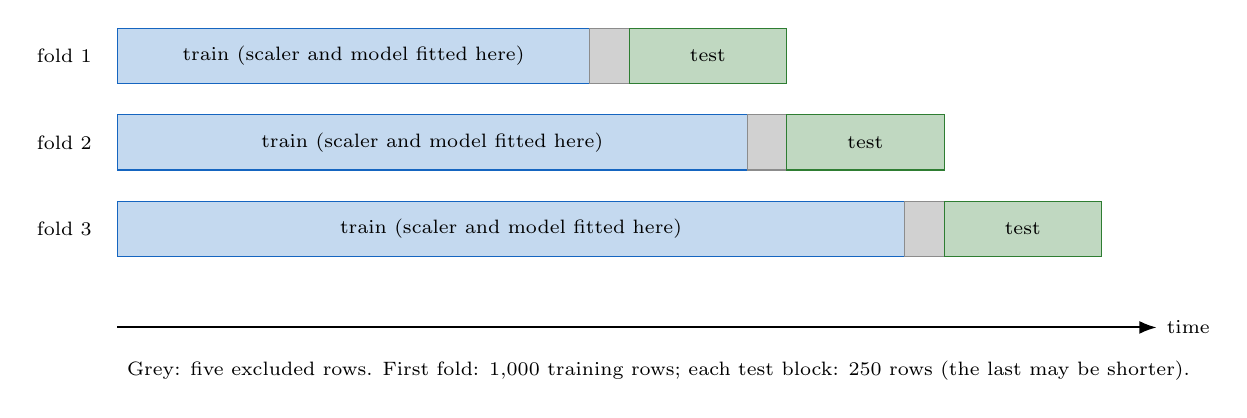
\begin{tikzpicture}[x=1mm,y=1mm]
\foreach \k/\tr in {1/60, 2/80, 3/100}{
  \pgfmathsetmacro{\yy}{-(\k-1)*11}
  \pgfmathsetmacro{\eb}{\tr+5}
  \pgfmathsetmacro{\tb}{\tr+25}
  \node[font=\scriptsize,anchor=east] at (-2,\yy+3.5) {fold \k};
  \draw[fill=cData!25,draw=cData] (0,\yy) rectangle (\tr,\yy+7);
  \node[font=\scriptsize] at (\tr/2,\yy+3.5) {train (scaler and model fitted here)};
  \draw[fill=black!18,draw=black!45] (\tr,\yy) rectangle (\eb,\yy+7);
  \draw[fill=cGood!30,draw=cGood] (\eb,\yy) rectangle (\tb,\yy+7);
  \node[font=\scriptsize] at (\eb+10,\yy+3.5) {test};
}
\draw[arr] (0,-31) -- (132,-31) node[right,font=\scriptsize] {time};
\node[font=\scriptsize,anchor=north west] at (0,-34)
  {Grey: five excluded rows. First fold: $1{,}000$ training rows; each test block: 250 rows (the last may be shorter).};
\end{tikzpicture}}
\caption{Expanding-window walk-forward evaluation. The training window grows by 250
rows per fold, and the scaler and classifier are refitted inside each fold on its
training rows only.}
\label{fig:wf}
\end{figure}

Within each fold, a standard scaler and a classifier are fitted together as one
pipeline on the training rows, and the pipeline is saved. The scaler is never
refitted at prediction time. The main model is an $\ell_2$-regularized logistic
regression (inverse penalty $C=0.1$, with intercept, at most $2{,}000$ iterations).
The second model is a histogram gradient-boosted tree classifier (depth 3, 200
iterations, learning rate $0.05$, $\ell_2$ leaf regularization 1, no early stopping,
seed 0). A logistic regression that sees only $\log(C_t/C_{t-1})$ is used as an
ablation. A forecast is ``up'' when the predicted probability is above $0.5$. The
hyperparameters were fixed in advance and kept the same across assets and folds,
and none of them was tuned on test data. The study is retrospective and was not
preregistered. In total, the evaluation fits 72 pipelines (24 asset-folds times
three classifiers).

\subsection{Baselines}

All baselines are scored on exactly the same dates as the model.
\begin{itemize}
\item \textbf{Persistence} predicts that the next move repeats the latest completed
move, $\hat y_t=\mathbf{1}(C_t>C_{t-1})$.
\item \textbf{Inverse persistence} predicts the opposite,
$\hat y_t=1-\mathbf{1}(C_t>C_{t-1})$, so exactly one of these two rules is right on
any day. It captures one-day reversal, and in these data it turns out to be the
strongest simple benchmark.
\item \textbf{Training majority} predicts the more frequent class in the current
training fold. In practice it was long BTC and short DOGE all the time, and long
ETH on $88\%$ of days.
\item \textbf{Passive basket} is an equal-weight long position in the assets that
are available on each date, rebalanced daily. It is a return benchmark, not a
classifier.
\end{itemize}

\subsection{Statistical inference}\label{ssec:inference}

For per-asset hit rates we report Wilson intervals, a two-sided test against
$0.5$, and the Pesaran--Timmermann test of independence between predicted and
realized direction.

The comparison with inverse persistence is paired. For a model $M$ and inverse
persistence $I$, define
\begin{equation}
d_{j,t}=\mathbf{1}\bigl(\hat y^{M}_{j,t}=y_{j,t}\bigr)-\mathbf{1}\bigl(\hat y^{I}_{j,t}=y_{j,t}\bigr).
\label{eq:diff}
\end{equation}
For each asset we estimate the mean of $d$ with a Bartlett-kernel HAC variance,
\begin{equation}
\widehat{\operatorname{Var}}(\bar d)=\frac{1}{n}\Bigl[\hat\gamma_0+2\sum_{\ell=1}^{K}\Bigl(1-\frac{\ell}{K+1}\Bigr)\hat\gamma_\ell\Bigr],
\qquad
\hat\gamma_\ell=\frac{1}{n}\sum_{t=\ell+1}^{n}v_t v_{t-\ell},
\qquad K=20,
\label{eq:hac}
\end{equation}
where $v_t=d_t-\bar d$, and we report normal-approximation intervals and two-sided
$p$-values.

For pooled statistics, Sharpe ratios and costs we use a circular stationary
bootstrap with $2{,}000$ replicates, a mean block length of 20 days and seed
$20{,}260{,}401$. Block lengths of 5 and 60 days are used as sensitivity checks. The
bootstrap resamples dates, not asset-days. In each replicate one sequence of date
indices is drawn and applied to every asset, including the mask that records which
assets are active, so the dependence between assets on the same day is kept. Pooled
accuracy and the pooled paired difference are computed again in each replicate as
ratios of sums over the sampled dates. Forecasts are not refitted inside the
replicates, so the intervals are conditional on the fitted walk-forward
predictions. We report percentile intervals, and we treat secondary comparisons as
exploratory.

\subsection{Economic evaluation}\label{ssec:econ}

\paragraph{Target-notional book} On date $t$, let $A_t$ be the set of assets with a
forecast and $J_t=|A_t|$. Each active asset gets the target weight
$w_{j,t}=s_{j,t}/J_t$, with $s_{j,t}=2\hat y_{j,t}-1\in\{-1,+1\}$, and inactive
assets get zero. Then
\begin{equation}
g_{t+1}=\sum_j w_{j,t}\,r_{j,t+1},\qquad
q_t=\sum_j\bigl|w_{j,t}-w_{j,t-1}\bigr|,\qquad
n_{t+1}(c)=g_{t+1}-c\,q_t,
\label{eq:book}
\end{equation}
where $r_{j,t+1}=C_{t+1}/C_t-1$. Weights start at zero, and the turnover of the
last day includes closing the book. Reversing the position in one asset costs two
units of turnover, and positions that keep their sign are carried over without
trading. The reference cost is $c=9$ basis points (bps) per unit of one-way
turnover. It is made up of a 4-bps taker fee and 5 bps of slippage, and
Section~\ref{ssec:costs} reports the whole cost curve. The book is directional and
does not need to be market neutral.

Sharpe ratios are annualized with 365 periods, the sample standard deviation and a
zero risk-free rate, and we also report annualized arithmetic means and
volatilities. In this linear book, the cost at which the mean net return is zero is
\begin{equation}
c^{*}=10^{4}\,\bar g/\bar q\ \text{bps},\qquad \bar q>0.
\label{eq:root}
\end{equation}
Each bootstrap replicate resamples $g$ and $q$ together and computes $c^{*}$ and
both Sharpe ratios again, so the uncertainty about turnover is included in the
interval. Values below zero are kept and not clipped.

\paragraph{Cash ledger} The second calculation is an explicit cash account with an
execution rule that is conservative on purpose. A forecast made at the close of $t$
is entered at the open of $t+1$ and closed at the close of $t+1$. This happens every
day, even when the next forecast points in the same direction, so the ledger pays a
full round trip on each asset every day. Each asset gets $1/J_t$ of the equity at
the start of the day. For side $s\in\{-1,+1\}$, slippage $\lambda=5$ bps and fee
rate $f=4$ bps,
\begin{equation}
\begin{aligned}
&P_{\text{in}}=O_{t+1}(1+s\lambda),\qquad P_{\text{out}}=C_{t+1}(1-s\lambda),\\
&R=s\Bigl(\frac{P_{\text{out}}}{P_{\text{in}}}-1\Bigr)-f\Bigl(1+\frac{P_{\text{out}}}{P_{\text{in}}}\Bigr).
\end{aligned}
\label{eq:ledger}
\end{equation}
The ledger books the entry and exit cash flows and the fee of each leg separately,
and it checks them against \eqref{eq:ledger}. Positions are flat at every close, the
account starts with $10{,}000$ units, and the Sharpe ratio uses only the $2{,}083$
evaluation days. Figure~\ref{fig:timing} shows how the return windows line up.

\begin{figure}[htbp]\centering
\resizebox{0.92\textwidth}{!}{%
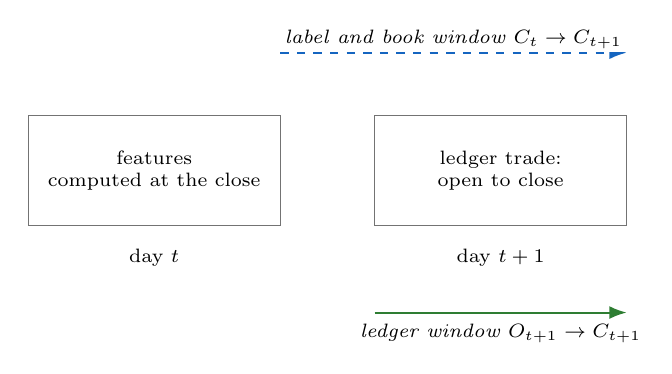
\begin{tikzpicture}[x=1mm,y=1mm]
\draw[draw=black!55] (0,0)  rectangle (32,14);
\draw[draw=black!55] (44,0) rectangle (76,14);
\node[font=\scriptsize] at (16,-4) {day $t$};
\node[font=\scriptsize] at (60,-4) {day $t+1$};
\node[font=\scriptsize,align=center] at (16,7) {features\\ computed at the close};
\node[font=\scriptsize,align=center] at (60,7) {ledger trade:\\ open to close};
\draw[arr,draw=cData,dashed] (32,22) -- node[lbl,above]{label and book window $C_t\to C_{t+1}$} (76,22);
\draw[arr,draw=cGood] (44,-11) -- node[lbl,below,yshift=-1mm]{ledger window $O_{t+1}\to C_{t+1}$} (76,-11);
\end{tikzpicture}}
\caption{Return windows. Because each day opens within a few basis points of the
previous close, $O_{t+1}\approx C_t$ and the ledger window closely tracks the label
window.}
\label{fig:timing}
\end{figure}

\subsection{Reproducibility}

Every number in this paper comes from deterministic scripts. One command rebuilds
the 72 pipelines, writes the $5{,}562$ dated forecasts with their fold identifiers,
probabilities and baseline decisions, computes all tables and the supplementary
diagnostics, reconciles the trade ledger, and runs the regression and mutation
suites (\ref{app:replication}).

%==============================================================================
\section{Results}\label{sec:results}
%==============================================================================

\subsection{Directional accuracy}

\begin{table}[htbp]\centering\small
\caption{Out-of-sample directional accuracy (\%). Pooled values are shares of
correct asset-days.}
\label{tab:acc}
\begin{tabular}{@{}lrrrr@{}}
\toprule
Predictor & BTC & ETH & DOGE & Pooled \\
\midrule
\textbf{Logistic regression} & $\mathbf{52.71}$ & $\mathbf{53.10}$ & $\mathbf{53.08}$ & $\mathbf{52.95}$ \\
Boosted trees                & $52.09$ & $51.37$ & $51.93$ & $51.78$ \\
Lag-1 logistic (ablation)    & $51.90$ & $52.66$ & $52.58$ & $52.36$ \\
Inverse persistence          & $53.00$ & $52.57$ & $53.15$ & $52.88$ \\
Persistence                  & $47.00$ & $47.43$ & $46.85$ & $47.12$ \\
Training majority            & $50.55$ & $49.59$ & $51.72$ & $50.49$ \\
\midrule
Forecasts ($n$)              & $2{,}083$ & $2{,}083$ & $1{,}396$ & $5{,}562$ \\
\bottomrule
\end{tabular}
\end{table}

Table~\ref{tab:acc} reports the out-of-sample accuracy of every predictor. Logistic
regression is the most accurate of the learned models. It is correct on $52.95\%$
of the $5{,}562$ asset-days, and the date-synchronized bootstrap puts the $95\%$
interval for this pooled number at $51.45$--$54.41\%$. This is clearly above one
half, even after we allow for the dependence between assets. The result also holds
for each asset. The Wilson intervals are $[50.6, 54.8]$, $[50.9, 55.2]$ and
$[50.5, 55.7]$ for BTC, ETH and DOGE, and the Pesaran--Timmermann test rejects
independence of predicted and realized direction with $p$-values of $0.015$,
$0.008$ and $0.016$. Logistic regression is more accurate than gradient-boosted
trees on all three assets. This suggests that, with a modest single-asset feature
set, the extra flexibility of trees does not help much.

\subsection{Comparison with the reversal benchmark}

\begin{table}[htbp]\centering\small
\caption{Paired accuracy differences against inverse persistence on identical
dates, in percentage points. A positive difference favors the model. Per-asset
intervals use a 20-lag Bartlett HAC variance; the pooled interval uses the
date-synchronized stationary bootstrap (mean block length 20).}
\label{tab:paired}
\begin{tabular}{@{}llrcr@{}}
\toprule
Asset & Model & Difference & 95\% interval & $p$ \\
\midrule
BTC  & Logistic       & $-0.29$ & $[-2.55,\ 1.97]$ & $0.803$ \\
BTC  & Boosted trees  & $-0.91$ & $[-3.03,\ 1.21]$ & $0.399$ \\
BTC  & Lag-1 logistic & $-1.10$ & $[-3.31,\ 1.10]$ & $0.327$ \\
\midrule
ETH  & Logistic       & $+0.53$ & $[-1.85,\ 2.91]$ & $0.663$ \\
ETH  & Boosted trees  & $-1.20$ & $[-3.73,\ 1.33]$ & $0.353$ \\
ETH  & Lag-1 logistic & $+0.10$ & $[-1.87,\ 2.06]$ & $0.924$ \\
\midrule
DOGE & Logistic       & $-0.07$ & $[-2.69,\ 2.55]$ & $0.957$ \\
DOGE & Boosted trees  & $-1.22$ & $[-3.84,\ 1.41]$ & $0.363$ \\
DOGE & Lag-1 logistic & $-0.57$ & $[-1.91,\ 0.76]$ & $0.399$ \\
\midrule
Pooled & Logistic     & $+0.07$ & $[-1.44,\ 1.61]$ & -- \\
\bottomrule
\end{tabular}
\end{table}

Next, the framework asks whether the model knows more than a rule with no
parameters. Inverse persistence is correct on $52.88\%$ of asset-days, which is
almost the same as the model, and Table~\ref{tab:paired} compares the two on paired
observations. The logistic model is ahead on ETH by $0.53$ points and within $0.3$
points on BTC and DOGE. The pooled difference is $+0.07$ points, with a $95\%$
interval from $-1.44$ to $1.61$, and the interval hardly changes with five-day or
sixty-day blocks (Table~\ref{tab:book}). So in terms of accuracy, the model and the
reversal rule cannot be separated. We see this as a finding about the data and not
as a weakness of the model. In daily cryptocurrency returns, much of the predictable
direction is one-day reversal, and a well-regularized model finds it without being
told to. The next two subsections show what the model learns beyond that rule and
where its forecasts add value.

\subsection{What the model learns}\label{ssec:learned}

The logistic model agrees with inverse persistence on $70.8\%$ of asset-days
($69.1\%$ for BTC, $71.1\%$ for ETH and $73.0\%$ for DOGE). Table~\ref{tab:coef}
shows the reason. Three of the features describe the move of the same day: the
one-day log return, the open-to-close return and the position of the close within
the day's range. For BTC and ETH all three have negative coefficients in every fold.
The close location has the largest weight of all 30 features for BTC ($-0.17$) and
the second largest for ETH ($-0.13$). These features overlap a lot. The one-day and
open-to-close returns have correlations of $0.998$, $0.997$ and $0.915$ for BTC,
ETH and DOGE, because each day opens within a few basis points of the previous
close, and the close location is correlated with both (about $0.7$ for BTC and
ETH). So their coefficients are best read together, as a regularized description
of one reversal signal. For DOGE the same signal shows up as the largest weight of
any feature, a negative one on the one-day return ($-0.42$), which is partly offset
by a positive weight on the open-to-close return ($+0.26$).

\begin{table}[htbp]\centering\small
\caption{Selected standardized logistic coefficients, averaged over folds. In
parentheses: the number of folds in which the coefficient has the same sign as its
average. Features are standardized within each training fold, so magnitudes are
comparable within a column.}
\label{tab:coef}
\begin{tabular}{@{}lrrr@{}}
\toprule
Feature & BTC (9 folds) & ETH (9 folds) & DOGE (6 folds) \\
\midrule
One-day log return               & $-0.045$ (9) & $-0.100$ (9) & $-0.415$ (6) \\
Open-to-close return             & $-0.042$ (9) & $-0.073$ (9) & $+0.259$ (6) \\
Close location in day's range    & $-0.174$ (9) & $-0.132$ (9) & $+0.011$ (4) \\
Three-day log return             & $+0.035$ (9) & $+0.056$ (8) & $+0.248$ (6) \\
Close $z$-score (60 days)        & $+0.126$ (9) & $+0.039$ (9) & $+0.023$ (5) \\
Average trade size               & $-0.131$ (9) & $+0.001$ (4) & $-0.053$ (6) \\
Normalized ATR (14 days)         & $+0.038$ (8) & $+0.187$ (9) & $-0.053$ (6) \\
Trade-count $z$-score (60 days)  & $-0.058$ (7) & $+0.130$ (9) & $-0.079$ (5) \\
Weekday, $\cos(2\pi d/7)$        & $-0.057$ (9) & $-0.075$ (9) & $-0.128$ (6) \\
\bottomrule
\end{tabular}
\end{table}

Beyond reversal, the model also uses information that the reversal rule cannot
see. The three-day return has a positive sign for every asset (in 23 of the 24
asset-folds), which is a mild continuation over several days. For BTC, the second
and third largest weights go to average trade size (negative) and to the close
relative to its 60-day mean (positive), each with the same sign in every fold. For
ETH, the largest weight of all goes to normalized ATR, and the trade-count
$z$-score ranks third. A weekly seasonal term is negative for every asset in every
fold. These terms are what make the forecasts of the model different from the
reversal rule on the other $29\%$ of asset-days.

\subsection{Where the model adds value: magnitude}\label{ssec:magnitude}

Directional accuracy gives a $0.2\%$ day the same weight as a $12\%$ day, so it is
a poor guide to profit in a market that is this volatile.
Table~\ref{tab:magnitude} looks at the size of the moves.

\begin{table}[htbp]\centering\small
\caption{Accuracy and magnitude. Panel A: accuracy (\%) by within-asset tercile of
the absolute next-day return, all assets pooled. Panel B: return-weighted hit rate
(\%), $\sum_t|r_t|\mathbf{1}(\text{correct}_t)/\sum_t|r_t|$, and the gross
annualized Sharpe ratio of a single-asset position that is long when the forecast
is up and short otherwise.}
\label{tab:magnitude}
\begin{tabular}{@{}lrrrrrr@{}}
\toprule
\multicolumn{7}{@{}l}{\emph{Panel A. Accuracy by size of the next-day move}} \\
\midrule
 & \multicolumn{2}{c}{Small} & \multicolumn{2}{c}{Medium} & \multicolumn{2}{c}{Large} \\
\cmidrule(lr){2-3}\cmidrule(lr){4-5}\cmidrule(l){6-7}
Asset-days & \multicolumn{2}{c}{$1{,}856$} & \multicolumn{2}{c}{$1{,}853$} & \multicolumn{2}{c}{$1{,}853$} \\
Logistic regression & \multicolumn{2}{c}{$52.9$} & \multicolumn{2}{c}{$54.9$} & \multicolumn{2}{c}{$\mathbf{51.1}$} \\
Inverse persistence & \multicolumn{2}{c}{$54.5$} & \multicolumn{2}{c}{$55.3$} & \multicolumn{2}{c}{$48.9$} \\
\midrule
\multicolumn{7}{@{}l}{\emph{Panel B. Magnitude-aware measures by asset}} \\
\midrule
 & \multicolumn{3}{c}{Return-weighted hit rate} & \multicolumn{3}{c}{Gross Sharpe ratio} \\
\cmidrule(lr){2-4}\cmidrule(l){5-7}
Predictor & BTC & ETH & DOGE & BTC & ETH & DOGE \\
\midrule
Logistic regression & $\mathbf{51.7}$ & $\mathbf{51.6}$ & $\mathbf{52.3}$ & $+0.44$ & $+0.42$ & $\mathbf{+0.61}$ \\
Lag-1 logistic      & $52.6$ & $52.6$ & $47.1$ & $+0.67$ & $+0.69$ & $-0.77$ \\
Inverse persistence & $51.1$ & $50.9$ & $47.0$ & $+0.30$ & $+0.25$ & $-0.79$ \\
Persistence         & $48.9$ & $49.1$ & $53.0$ & $-0.30$ & $-0.25$ & $+0.79$ \\
\bottomrule
\end{tabular}
\end{table}

Panel~A splits the evaluation days of each asset into terciles of the absolute
next-day return. The reversal rule does better on small and medium days, but on the
largest third of days the model is correct $51.1\%$ of the time, against $48.9\%$
for the rule. Panel~B shows what this means for returns. The model has a higher
return-weighted hit rate than the reversal rule on all three assets, and it is the
only rule in the panel whose single-asset gross Sharpe ratio is positive on every
asset: $0.44$ for BTC, $0.42$ for ETH and $0.61$ for DOGE. The reversal rule, on the
other hand, loses money on DOGE. There its return-weighted hit rate is $47.0\%$ and
its gross Sharpe ratio is $-0.79$, even with a $53.2\%$ hit rate, so on DOGE
accuracy and returns rank the two rules in opposite orders. The lag-1 ablation,
which uses only reversal, shows the same pattern. This suggests that the additional
terms of the model (Section~\ref{ssec:learned}) are what keep it on the right side
of the large moves of DOGE.

The same pattern holds in the portfolio. The logistic book has a gross Sharpe ratio
of $0.54$ and the inverse-persistence book has $0.004$ (Table~\ref{tab:variants}).
When dates are resampled jointly, the annualized gross mean of the logistic book is
higher than that of the reversal book by $31.5$ percentage points. The $95\%$
interval, from $-15.0$ to $+76.9$, is wide, so the size of the advantage is
uncertain, but its direction is the same in all the magnitude measures.

\subsection{Stability across folds}

Accuracy changes with market conditions (\ref{app:folds}). For the logistic model
it reaches $61.6\%$ in the fifth fold of ETH (April to December 2023) and $59.2\%$
in the sixth fold of BTC (December 2023 to August 2024), and it ranges from
$42.2\%$ to $61.6\%$ across the 24 asset-folds. The most recent folds, which are
also the shortest (83 days for BTC and ETH and 146 for DOGE), are the weakest for
both the model and the reversal rule. So a pooled number is an average over quite
different regimes, and we publish the fold-level record together with the results.

\subsection{Economic performance}\label{ssec:costs}

\begin{table}[htbp]\centering\small
\caption{Target-notional book for the logistic forecasts. Panel A: point estimates
at 9 bps per unit of one-way turnover over $2{,}083$ dates. Panel B: 95\% percentile
intervals from the date-synchronized stationary bootstrap ($2{,}000$ replicates) for
three mean block lengths; 20 days is the primary choice. The accuracy difference is
against inverse persistence, in percentage points.}
\label{tab:book}
\begin{tabular}{@{}lrrrr@{}}
\toprule
\multicolumn{5}{@{}l}{\emph{Panel A. Point estimates}} \\
\midrule
 & Annualized mean & Volatility & Sharpe ratio & \\
\midrule
Gross & $31.7\%$ & $58.4\%$ & $0.544$ & \\
Net   & $6.6\%$  & $58.4\%$ & $0.113$ & \\
\midrule
\multicolumn{5}{@{}l}{Turnover $0.766$ a day; cost $6.89$ bps a day; break-even cost $c^{*}=11.36$ bps.} \\
\midrule
\multicolumn{5}{@{}l}{\emph{Panel B. 95\% intervals by mean block length}} \\
\midrule
Block & Accuracy diff. & Gross Sharpe & Net Sharpe & Break-even (bps) \\
\midrule
5 days  & $[-1.49,\ 1.62]$ & $[-0.27,\ 1.30]$ & $[-0.69,\ 0.86]$ & $[-5.68,\ 26.95]$ \\
20 days & $[-1.44,\ 1.61]$ & $[-0.19,\ 1.32]$ & $[-0.60,\ 0.87]$ & $[-4.00,\ 26.43]$ \\
60 days & $[-1.47,\ 1.56]$ & $[-0.14,\ 1.30]$ & $[-0.56,\ 0.84]$ & $[-3.06,\ 25.78]$ \\
\bottomrule
\end{tabular}
\end{table}

Table~\ref{tab:book} reports the target-notional book for the logistic forecasts.
Before costs it earns an annualized mean of $31.7\%$ with a volatility of $58.4\%$,
which is a Sharpe ratio of $0.544$. Turnover is $0.766$ units a day on average, so
at 9 bps the cost is $6.89$ bps a day. This leaves a net mean of $6.6\%$ and a net
Sharpe ratio of $0.113$. The break-even cost is $11.4$ bps per unit of turnover,
which is above the 9 bps that we assume, so the strategy stays profitable in the
point estimate at realistic fee and slippage levels (Figure~\ref{fig:cost}). The
bootstrap intervals are wide: $-0.19$ to $1.32$ for the gross Sharpe ratio, $-0.60$
to $0.87$ for the net Sharpe ratio and $-4.0$ to $26.4$ bps for the break-even
cost. They change little with the block length. This is what we should expect from
$2{,}083$ daily observations, for which a Sharpe ratio of $0.54$ has a standard
error of roughly $0.38$, and it is the reason why the framework gives an interval
for every economic quantity.

\begin{figure}[htbp]\centering
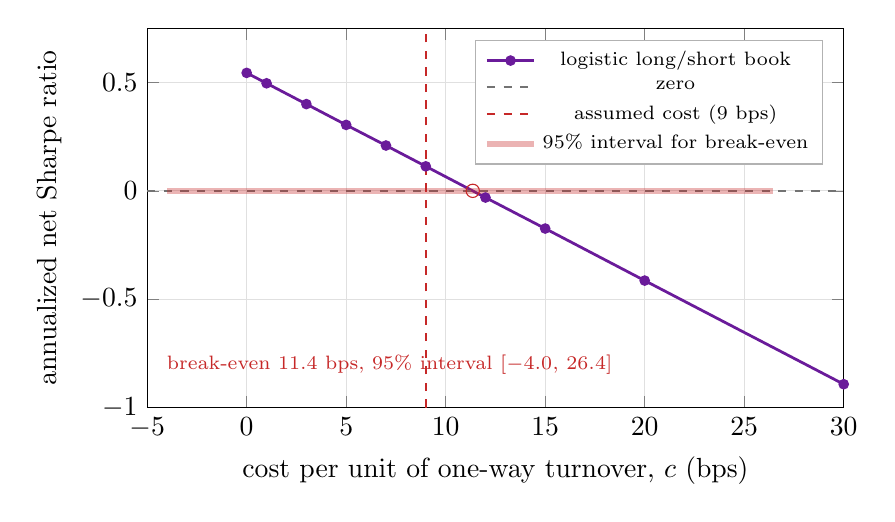
\begin{tikzpicture}
\begin{axis}[width=0.86\textwidth,height=6.4cm,
    xlabel={cost per unit of one-way turnover, $c$ (bps)},
    ylabel={annualized net Sharpe ratio},
    xmin=-5,xmax=30,ymin=-1.0,ymax=0.75,
    grid=major,grid style={black!12},
    legend pos=north east,legend style={font=\scriptsize,draw=black!30}]
\addplot[color=cEval,mark=*,mark size=1.4pt,line width=1pt] coordinates {
  (0,0.544) (1,0.496) (3,0.400) (5,0.304) (7,0.209)
  (9,0.113) (12,-0.031) (15,-0.174) (20,-0.414) (30,-0.892)};
\addlegendentry{logistic long/short book}
\addplot[color=black!55,dashed,line width=0.7pt] coordinates {(-5,0) (30,0)};
\addlegendentry{zero}
\addplot[color=cBad,dashed,line width=0.9pt] coordinates {(9,-1.0) (9,0.75)};
\addlegendentry{assumed cost (9 bps)}
\addplot[color=cBad,line width=2.2pt,opacity=0.35] coordinates {(-4.00,0) (26.43,0)};
\addlegendentry{95\% interval for break-even}
\addplot[color=cBad,only marks,mark=o,mark size=2.4pt,forget plot] coordinates {(11.36,0)};
\node[font=\scriptsize,anchor=west,text=cBad] at (axis cs:-4.5,-0.8)
     {break-even $11.4$ bps, 95\% interval $[-4.0,\,26.4]$};
\end{axis}
\end{tikzpicture}
\caption{Net Sharpe ratio of the logistic book as a function of the cost per unit of
turnover. The curve is a set of point estimates, not a confidence band; the shaded
segment is the bootstrap interval for the break-even cost.}
\label{fig:cost}
\end{figure}

\subsection{Policy variants}

\begin{table}[htbp]\centering\small
\caption{Target-notional book for every predictor and two variants of the logistic
policy, at 9 bps per unit of turnover. Intervals were computed for the primary
logistic book (Table~\ref{tab:book}); the remaining rows are descriptive.}
\label{tab:variants}
\begin{tabular}{@{}lrrrr@{}}
\toprule
Policy & Dates & Gross Sharpe & Net Sharpe & Turnover \\
\midrule
\textbf{Logistic regression}        & $2{,}083$ & $\mathbf{+0.544}$ & $\mathbf{+0.113}$ & $0.766$ \\
Boosted trees                       & $2{,}083$ & $+0.234$ & $-0.216$ & $0.770$ \\
Lag-1 logistic                      & $2{,}083$ & $+0.386$ & $-0.057$ & $0.817$ \\
Inverse persistence                 & $2{,}083$ & $+0.004$ & $-0.547$ & $1.060$ \\
Persistence                         & $2{,}083$ & $-0.004$ & $-0.555$ & $1.060$ \\
Training majority                   & $2{,}083$ & $+0.112$ & $+0.110$ & $0.002$ \\
\midrule
Logistic, three-asset dates         & $1{,}396$ & $+0.947$ & $+0.473$ & $0.755$ \\
Logistic, long or cash              & $2{,}083$ & $+0.964$ & $+0.712$ & $0.383$ \\
\bottomrule
\end{tabular}
\end{table}

Table~\ref{tab:variants} applies the same book to every predictor and to two
variants of the logistic policy. Among the predictors, logistic regression has both
the highest gross and the highest net Sharpe ratio. Its closest rival on a net basis
is the training-majority rule. This rule is in effect a static allocation (long
BTC, short DOGE and mostly long ETH) with almost no turnover. Boosted trees, the
lag-1 ablation and both persistence rules all earn less before costs or trade more,
and the persistence rules, which reverse their position on $53\%$ of days, are hit
hardest by costs. Two variants improve the logistic book further. If we restrict it
to the $1{,}396$ dates on which all three assets are active, the net Sharpe ratio
rises to $0.47$. A long-or-cash version that never sells short reaches $0.71$ with
half the turnover, and it holds a position on $56\%$ of asset-days. For context,
the fully invested passive basket had a gross Sharpe ratio of $0.92$ over this
strongly rising period. Confidence gating, which trades only when the predicted
probability is far from one half, lowers turnover, but it did not raise the net
Sharpe ratio in this sample (\ref{app:sensitivity}).

\subsection{Execution policy}\label{ssec:ledger}

The cash ledger gives a second view of implementation, which is conservative on
purpose. Before costs, the logistic forecasts point the right way on $52.9\%$ of
next-day open-to-close moves and capture $9.9$ bps per trade on average. So the
forecasting edge carries over from the close-to-close label window to an
open-to-close window that can be traded. However, the ledger closes and reopens
every position every day, so it pays about 18 bps per asset-day in slippage and
fees, against $6.9$ bps a day for the netted book. At this rate the edge is used up:
the net return per trade is $-8.1$ bps and the Sharpe ratio of the ledger is
$-0.58$. This comparison is useful. Entry timing costs almost nothing, because each
day opens within a few basis points of the previous close. Over the evaluation
window the standard deviation of the close-to-next-open return is $0.6$, $0.9$ and
$3.5$ bps for BTC, ETH and DOGE, against $306$, $415$ and $1{,}084$ bps for the
open-to-close return. What decides whether the forecasts can be traded is whether
the execution rule nets consecutive positions, as the target-notional book does.
The ledger is also an accounting check. Its cash reconciles with the trade records
to within $5\times10^{-12}$ units on every day, and every position is flat at the
close.

\subsection{Relation to passive exposure}\label{ssec:bench}

A directional long/short book should not be ranked against a long-only holding by
raw Sharpe ratios. What matters is how the two work together. When we regress the
net daily return of the logistic book on the passive basket, we get a beta of
$0.17$ and a correlation of $0.20$. So the strategy has little market exposure, and
it is a natural candidate for diversification. Its regression intercept is small
and not statistically different from zero ($t=-0.18$ with a 20-lag HAC standard
error). Over this sample, its contribution to a passive holding is therefore mainly
diversification, not a measurable stand-alone alpha.

%==============================================================================
\section{Verification of the implementation}\label{sec:verification}
%==============================================================================

The number of tests shows effort, but what matters is whether the tests find the
failures they were written for. The test suite for the backtest engine and the
feature pipeline has 29 tests. They cover next-bar entry, asset-specific pricing,
short valuation, intrabar stops, the holding rule, annualization, resampling, cash
reconciliation, scaler persistence and split gaps. The research code adds 22 more
checks, for example a hand-computed HAC variance, rejection of degenerate inputs,
the exact cost root, own-notional fees, the feature count and prefix invariance,
and reconciliation of the saved models, forecasts and results. All 51 tests pass.

For mutation testing we put back one contract violation at a time and run the
29-test suite again. A mutant counts as detected only if the test written for that
contract fails, the number of tests that ran is the same as in the baseline, and
the exit status agrees. Collection errors and skipped tests do not count as
detection. Table~\ref{tab:mutation} shows that all eight mutants are detected. The
other two contracts, next-bar fills (C2) and asset-specific pricing (C4), cannot be
violated on their own without rewriting the simulation loop, so each of them is
protected by a dedicated test instead. Because we chose the eight mutants
ourselves, the score is evidence about these contracts and not about every
possible defect.

\begin{table}[htbp]\centering\footnotesize
\caption{Mutation testing. Each row re-inserts one contract violation into the
engine and reruns the 29-test suite. ``Failed'' is the number of tests that fail;
the named test is the one that must fail for the mutant to count as detected.}
\label{tab:mutation}
\begin{tabular}{@{}lL{0.27\textwidth}L{0.47\textwidth}r@{}}
\toprule
Contract & Re-inserted violation & Test that must fail & Failed \\
\midrule
C1  & Nearest bar, possibly in the future & \texttt{price\_\allowbreak lookup\_\allowbreak never\_\allowbreak selects\_\allowbreak a\_\allowbreak future\_\allowbreak bar} & 1 \\
C3  & Stops checked at the close only & \texttt{stop\_\allowbreak wins\_\allowbreak when\_\allowbreak one\_\allowbreak bar\_\allowbreak touches\_\allowbreak both\_\allowbreak levels} & 2 \\
C5  & Short valued with the wrong sign & \texttt{short\_\allowbreak equity\_\allowbreak falls\_\allowbreak when\_\allowbreak price\_\allowbreak rises} & 1 \\
C6  & Fee split evenly across legs & \texttt{equity\_\allowbreak curve\_\allowbreak reconciles\_\allowbreak with\_\allowbreak summed\_\allowbreak trade\_\allowbreak pnl} & 1 \\
C7  & Per-trade annualization & \texttt{annualisation\_\allowbreak matches\_\allowbreak the\_\allowbreak closed\_\allowbreak form} & 2 \\
C8  & Permutation used as resampling & \texttt{bootstrap\_\allowbreak is\_\allowbreak not\_\allowbreak degenerate} & 1 \\
C9  & Scaler refitted at inference & \texttt{single\_\allowbreak row\_\allowbreak transform\_\allowbreak is\_\allowbreak not\_\allowbreak all\_\allowbreak zeros} & 2 \\
C10 & Gap between folds removed & \texttt{gap\_\allowbreak between\_\allowbreak folds\_\allowbreak is\_\allowbreak at\_\allowbreak least\_\allowbreak the\_\allowbreak sequence\_\allowbreak length} & 2 \\
\midrule
\multicolumn{3}{@{}l}{\textbf{Mutation score}} & $\mathbf{8/8}$ \\
\bottomrule
\end{tabular}
\end{table}

The pipeline can also be reproduced on different platforms. A clean re-run in a
new Windows environment with Python 3.12 reproduced the primary output files byte
for byte. A re-run on Linux with Python 3.13 and newer library versions reproduced
every forecast and table, and the differences in predicted probabilities were below
$10^{-12}$. The input files are identified by SHA-256 hashes
(\ref{app:replication}).

%==============================================================================
\section{Discussion}\label{sec:discussion}
%==============================================================================

\subsection{What the framework reveals}

Three findings stand out, and each one depends on a layer of the framework that a
standard evaluation would leave out. The first comes from the baseline layer. A hit
rate of $52.95\%$ looks like a result of the model, but almost all of it is also
available to a rule with no parameters, and without the paired comparison nobody
would notice this. The second comes from the magnitude layer. What the model adds
over that rule is not how often it is right, but on which days it is right, and
accuracy alone cannot show this difference. On DOGE, accuracy even ranks the two
rules in the wrong order. The third comes from the economic layer. Whether a
forecasting edge can be traded depends on costs and on the execution rule as much
as on the forecast. The same forecasts earn a positive net Sharpe ratio when
positions are netted and a negative one when they are rebuilt every day.

\subsection{Statistical and economic significance}

The logistic hit rates are different from one half on every asset, but the
interval for the gross Sharpe ratio contains zero. Both statements are true.
Accuracy affects returns only through a small margin, $2a-1\approx0.06$, and
through which days happen to be called correctly, while costs take away an amount
that is proportional to turnover. With $2{,}083$ dates, a Sharpe ratio of $0.54$
has a bootstrap standard error of roughly $0.38$. Finding an effect and being paid
for it need different amounts of statistical power, and an evaluation should report
both.

\subsection{Practical guidance}

Table~\ref{tab:checklist} sums up the framework as a list of components, the
problem that each one protects against, and the evidence for it in this study. Each
component is cheap to use. Together they turn a single accuracy number into a clear
account of what a model knows, where its value comes from and what it would cost
to use it.

\begin{table}[htbp]\centering\small
\caption{Framework components, what each guards against, and the evidence in this
study.}
\label{tab:checklist}
\begin{tabular}{@{}L{0.32\textwidth}L{0.29\textwidth}L{0.31\textwidth}@{}}
\toprule
Component & Guards against & Evidence here \\
\midrule
Score persistence, inverse persistence and the majority class on identical dates & Crediting a model with an effect that a one-line rule captures & Reversal rule $52.88\%$, model $52.95\%$ \\
Paired, dependence-aware tests; resample dates, not asset-days & Overstated significance from correlated observations & Pooled accuracy interval $51.45$--$54.41\%$ \\
Magnitude-aware measures next to accuracy & Hit rates that hide where money is made & DOGE: reversal Sharpe $-0.79$, model $+0.61$ \\
Break-even cost estimated jointly with turnover; explicit execution rule & False precision about tradability & $11.4$ bps, interval $[-4.0, 26.4]$; netting versus daily rebuild \\
Engine rules as contracts, confirmed by mutation & Tests that accompany code without checking it & 8 of 8 violations detected \\
Rank-based provenance screen for external features & Price-derived features presented as external information & Sentiment proxy: rank correlation $0.95$--$0.97$ with same-day return \\
Dated forecasts and saved pipelines & Results that cannot be re-scored & $5{,}562$ forecasts; 72 pipelines \\
\bottomrule
\end{tabular}
\end{table}

%==============================================================================
\section{Limitations and future work}\label{sec:limitations}
%==============================================================================

The framework is general, but the evidence in this paper has a clear scope. It
covers three large assets that are still listed, on one exchange, with daily bars
that start at 00:00 UTC. Other assets, exchanges and bar boundaries still need to
be studied, and moving the start of the bars to other hours would show whether the
results depend on the boundary. The analysis is retrospective. The hyperparameters
were fixed in advance, but nothing was preregistered, so a prospective holdout is
the natural next step. The 30 features are single-asset technical measures.
Funding rates, open interest, basis, liquidations, order-book data and cross-asset
effects are clear extensions. Cost-aware training objectives and meta-labeling
\citep{lopezdeprado2018advances} are also possible, and meta-labeling targets
exactly the gap between direction and magnitude that we show in
Section~\ref{ssec:magnitude}. The HAC estimator and the stationary bootstrap allow
for short-range dependence, but not for every kind of regime shift, and the
bootstrap does not refit the models. Finally, the cost model is a flat 9 bps per
unit of turnover. Maker execution could make it lower for BTC and ETH, while
shorting on the spot market needs margin, and we do not model borrowing costs,
funding or capacity. The ratios in this paper are research diagnostics, not
expected returns for investors.

%==============================================================================
\section{Conclusion}\label{sec:conclusion}
%==============================================================================

We have built a tested, leakage-safe framework for evaluating machine-learning
forecasts of cryptocurrency returns, and we applied it to $5{,}562$ daily
out-of-sample forecasts for BTC, ETH and DOGE. A regularized logistic model is
correct $52.95\%$ of the time, with a dependence-robust interval that excludes one
half, and it beats a coin flip on every asset. The framework shows that much of
this directional skill is shared with one-day reversal, and that the special value
of the model is in magnitude. It gets more of the large moves right, it has the
higher return-weighted hit rate on every asset, and it earns a gross Sharpe ratio
of $0.54$ against $0.004$ for the reversal rule. At a realistic cost of 9 bps per
unit of turnover the netted strategy keeps a positive net Sharpe ratio of $0.11$,
its break-even cost is $11.4$ bps, and a long-or-cash version reaches $0.71$. The
intervals are wide, as we expect with less than six years of daily data.

The wider lesson is about evaluation. Accuracy, value beyond simple rules, value on
large moves and profit after costs are different questions, and each one needs its
own evidence. The framework answers all four with dated forecasts, inference that
allows for dependence, cost uncertainty, and an engine whose rules are checked by
tests that are themselves tested. Every number comes from one command and every
fitted model is saved, so the same process can be applied directly to richer
features, other assets and new models.

%==============================================================================
%  Declarations
%==============================================================================

\section*{Data and code availability}

The code, the three input files, the dated out-of-sample forecasts, the trade
ledger and all machine-readable results are kept in a public code repository. To
keep the review anonymous, its link is not shown in this copy. The link is given on
the separate title page, and it will be added to the paper after review.
The market data are public Binance kline archives. The complete analysis is rebuilt
by \texttt{python scripts/reproduce\_jfds.py}, and \ref{app:replication} lists the
software versions, random seeds and input-file hashes.

\section*{Declaration of generative AI and AI-assisted technologies}

\emph{AI use statement.} During the preparation of this work the authors used
OpenAI Codex and Anthropic Claude. We used these tools to help write and refactor
parts of the analysis code and tests, to suggest related literature, to draft and
revise parts of the manuscript, to check its wording, formatting and internal
consistency, and to compare the reported numbers with the outputs of the
replication scripts, which included running those scripts again. We did not use
generative AI to create, change or impute data, and no number in this paper was
produced by a language model. Every result comes from the deterministic scripts in
the replication package, which the authors ran and checked. An author reviewed all
code suggested by an AI tool before it was kept, and its behavior is checked by the
regression and mutation tests in Section~\ref{sec:verification}. The authors read
and verified every reference suggested by an AI tool before citing it. After using
these tools, the authors reviewed and edited the content as needed and take full
responsibility for the content of the publication, including all text, claims, code
and other material produced with the help of generative AI.

\section*{Ethics statement}

This study uses publicly available exchange price data and software written by the
authors. It does not involve human participants, personal data or animals, so
ethical approval and informed consent were not needed. The synthetic sentiment
series in Section~\ref{ssec:provenance} is a development placeholder, and its
generator script marks it as a price-based proxy. We use it here only to show how
the provenance screen works. Nothing in this paper is investment advice. Backtested
ratios like the ones in this paper are research diagnostics and not expected
returns, and trading cryptocurrencies has a high risk of loss. The main risk of
misuse that we see is that a strategy which passes the checks in this paper is
taken as proven to be profitable. Passing them is necessary, but it is not
sufficient.

\section*{Reproducibility statement}

We have tried to make every result in this paper easy to check. First, we provide
the source code for all experiments, together with the three input files, the dated
out-of-sample forecasts, the trade ledger and machine-readable results, and the
replication command rebuilds the 72 fitted fold pipelines. Second, the appendices
give the full feature definitions (\ref{app:features}), the fold boundaries and
fold-level results (\ref{app:folds}), the execution rules (\ref{app:execution}),
the cost and gating sensitivities (\ref{app:sensitivity}), and the commands,
software versions, random seeds and input-file hashes needed for replication
(\ref{app:replication}). Third, we state all datasets, models, hyperparameters and
hardware requirements, and we define each metric where it is first used. The whole
pipeline runs on an ordinary CPU in a few minutes, and it needs no GPU, database or
exchange account.

%==============================================================================
\appendix
%==============================================================================

\section{Feature definitions}\label{app:features}

Let $O,H,L,C,V,Q,N,B$ denote open, high, low and close prices, base volume, quote
volume, number of trades and taker-buy base volume. Let $\mu_k$ and $\sigma_k$ be
the trailing $k$-bar mean and sample standard deviation, and
$z_k(X)=(X-\mu_k(X))/\sigma_k(X)$. Every rolling window ends at $t$. Ratios with a
zero denominator are set to missing, and rows with any missing feature are dropped
before fitting (in practice only the warm-up rows).

\begin{table}[H]\centering\small
\caption{The 30 features.}
\label{tab:features}
\begin{tabular}{@{}L{0.22\textwidth}rL{0.62\textwidth}@{}}
\toprule
Group & Count & Definitions \\
\midrule
Log returns & 6 & $\log(C_t/C_{t-k})$ for $k\in\{1,2,3,5,10,20\}$ \\
Volatility and location & 8 & $\sigma_k\bigl(\log(C_t/C_{t-1})\bigr)$ and $z_k(C_t)$ for $k\in\{5,10,20,60\}$ \\
Bar shape & 3 & $(H_t-L_t)/C_t$, $(C_t-O_t)/O_t$, $(C_t-L_t)/(H_t-L_t)$ \\
Trading activity & 7 & $B_t/V_t$, $\mu_5(B/V)$, $Q_t/N_t$, $z_{60}(Q/N)$, $z_{60}(N)$, $z_{60}(V)$, $V_t/\mu_{20}(V)$ \\
Technical and calendar & 6 & RSI(14), MACD histogram, Bollinger position, normalized ATR(14), $\sin(2\pi d/7)$, $\cos(2\pi d/7)$ \\
\midrule
Total & 30 & \\
\bottomrule
\end{tabular}
\end{table}

With $\delta_t=C_t-C_{t-1}$, RSI is
$100-100/\bigl[1+\mu_{14}(\max(\delta,0))/\mu_{14}(\max(-\delta,0))\bigr]$, which
uses simple rolling means rather than Wilder's recursive smoothing. The MACD
histogram is $M-\mathrm{EMA}_9(M)$ with $M=\mathrm{EMA}_{12}(C)-\mathrm{EMA}_{26}(C)$;
exponential means use $\alpha=2/(k+1)$, start at the first observation and are not
bias-adjusted. Bollinger position is $(C_t-\mu_{20}(C))/(2\sigma_{20}(C))$. The
true range is $\max\{H_t-L_t,\,|H_t-C_{t-1}|,\,|L_t-C_{t-1}|\}$, and normalized ATR
is its 14-day simple mean divided by $C_t$. The weekday $d$ runs from 0 (Monday) to
6. The trading-activity fields summarize the day's trades; they are not order-book
snapshots.

\section{Fold boundaries and fold-level accuracy}\label{app:folds}

\begin{center}\small
\setlength{\tabcolsep}{4pt}
\begin{longtable}{@{}llrlllrrr@{}}
\caption{Fold boundaries and out-of-sample accuracy (\%) of the logistic model (L)
and inverse persistence (I). ``Last label'' is the date of the close that defines
the last training label; test dates are forecast dates.}
\label{tab:folds}\\
\toprule
Asset & Fold & Train rows & Last label & Test start & Test end & $n$ & L & I \\
\midrule
\endfirsthead
\toprule
Asset & Fold & Train rows & Last label & Test start & Test end & $n$ & L & I \\
\midrule
\endhead
\bottomrule
\endfoot
BTC  & 1 & 1,000 & 2020-07-12 & 2020-07-17 & 2021-03-23 & 250 & 50.0 & 55.6 \\
BTC  & 2 & 1,250 & 2021-03-19 & 2021-03-24 & 2021-11-28 & 250 & 50.4 & 55.6 \\
BTC  & 3 & 1,500 & 2021-11-24 & 2021-11-29 & 2022-08-05 & 250 & 51.6 & 50.8 \\
BTC  & 4 & 1,750 & 2022-08-01 & 2022-08-06 & 2023-04-12 & 250 & 51.6 & 54.0 \\
BTC  & 5 & 2,000 & 2023-04-08 & 2023-04-13 & 2023-12-18 & 250 & 54.8 & 54.8 \\
BTC  & 6 & 2,250 & 2023-12-14 & 2023-12-19 & 2024-08-24 & 250 & 59.2 & 54.8 \\
BTC  & 7 & 2,500 & 2024-08-20 & 2024-08-25 & 2025-05-01 & 250 & 55.2 & 52.0 \\
BTC  & 8 & 2,750 & 2025-04-27 & 2025-05-02 & 2026-01-06 & 250 & 52.0 & 50.0 \\
BTC  & 9 & 3,000 & 2026-01-02 & 2026-01-07 & 2026-03-30 & 83  & 43.4 & 42.2 \\
\midrule
ETH  & 1 & 1,000 & 2020-07-12 & 2020-07-17 & 2021-03-23 & 250 & 49.2 & 52.0 \\
ETH  & 2 & 1,250 & 2021-03-19 & 2021-03-24 & 2021-11-28 & 250 & 54.4 & 52.4 \\
ETH  & 3 & 1,500 & 2021-11-24 & 2021-11-29 & 2022-08-05 & 250 & 48.0 & 50.8 \\
ETH  & 4 & 1,750 & 2022-08-01 & 2022-08-06 & 2023-04-12 & 250 & 50.0 & 54.8 \\
ETH  & 5 & 2,000 & 2023-04-08 & 2023-04-13 & 2023-12-18 & 250 & 61.6 & 54.0 \\
ETH  & 6 & 2,250 & 2023-12-14 & 2023-12-19 & 2024-08-24 & 250 & 54.4 & 56.0 \\
ETH  & 7 & 2,500 & 2024-08-20 & 2024-08-25 & 2025-05-01 & 250 & 57.6 & 54.0 \\
ETH  & 8 & 2,750 & 2025-04-27 & 2025-05-02 & 2026-01-06 & 250 & 53.2 & 48.4 \\
ETH  & 9 & 3,000 & 2026-01-02 & 2026-01-07 & 2026-03-30 & 83  & 42.2 & 47.0 \\
\midrule
DOGE & 1 & 1,000 & 2022-05-30 & 2022-06-04 & 2023-02-08 & 250 & 55.6 & 58.8 \\
DOGE & 2 & 1,250 & 2023-02-04 & 2023-02-09 & 2023-10-16 & 250 & 58.0 & 57.6 \\
DOGE & 3 & 1,500 & 2023-10-12 & 2023-10-17 & 2024-06-22 & 250 & 52.8 & 53.6 \\
DOGE & 4 & 1,750 & 2024-06-18 & 2024-06-23 & 2025-02-27 & 250 & 52.4 & 51.2 \\
DOGE & 5 & 2,000 & 2025-02-23 & 2025-02-28 & 2025-11-04 & 250 & 48.8 & 49.2 \\
DOGE & 6 & 2,250 & 2025-10-31 & 2025-11-05 & 2026-03-30 & 146 & 49.3 & 45.2 \\
\end{longtable}
\end{center}

Training windows start on 16 October 2017 for BTC and ETH and on 3 September 2019
for DOGE, the first dates with a complete feature vector.

\section{Execution engine}\label{app:execution}

The backtest engine iterates over the union of bar timestamps. At each timestamp,
for every asset that has a bar, it first resolves exits for open positions in that
asset using that bar, then opens positions scheduled for that bar, and finally
closes positions whose bar-counted holding period ends at that bar's close. A
signal time-stamped within bar $i$ executes at bar $i+1$, at the open adjusted for
slippage, $p_{\text{entry}}=O_{i+1}(1\pm\varsigma)$. Cash and equity follow
\eqref{eq:equity}. A long entry debits $q\,p_{\text{entry}}+\varphi$ and a short
entry credits $q\,p_{\text{entry}}-\varphi$, where $\varphi$ is the fee on that
leg's own notional. Stops and targets are resolved against each bar's low and high;
when one bar touches both, the stop is assumed to fill first. Otherwise a position
closes at $C_t$ when its holding period expires. The cash ledger of
Section~\ref{ssec:econ} is a separate and simpler calculation that uses no
barriers.

\section{Cost curve and confidence gating}\label{app:sensitivity}

\begin{table}[H]\centering\small
\caption{Logistic book: mean daily net return and annualized net Sharpe ratio at
each cost per unit of one-way turnover.}
\label{tab:costcurve}
\begin{tabular}{@{}rrr@{}}
\toprule
Cost (bps) & Mean net return (bps a day) & Net Sharpe ratio \\
\midrule
0  & $8.70$   & $0.544$  \\
1  & $7.93$   & $0.496$  \\
3  & $6.40$   & $0.400$  \\
5  & $4.87$   & $0.304$  \\
7  & $3.34$   & $0.209$  \\
9  & $1.81$   & $0.113$  \\
12 & $-0.49$  & $-0.031$ \\
15 & $-2.79$  & $-0.174$ \\
20 & $-6.62$  & $-0.414$ \\
30 & $-14.27$ & $-0.892$ \\
\bottomrule
\end{tabular}
\end{table}

\begin{table}[H]\centering\small
\caption{Confidence gating at 9 bps. An asset keeps its $1/J_t$ allocation only when
$|p-0.5|\ge h$; otherwise that allocation stays in cash. No threshold is selected
from these results.}
\label{tab:gates}
\begin{tabular}{@{}lrrrrr@{}}
\toprule
Threshold $h$ & $0.00$ & $0.02$ & $0.04$ & $0.06$ & $0.08$ \\
\midrule
Net Sharpe ratio & $+0.113$ & $+0.018$ & $-0.080$ & $-0.191$ & $-0.309$ \\
Turnover         & $0.766$ & $0.736$ & $0.642$ & $0.522$ & $0.388$ \\
\bottomrule
\end{tabular}
\end{table}

\section{Replication details}\label{app:replication}

The analysis was developed with CPython 3.12.0, NumPy 2.4.4, pandas 3.0.3, SciPy
1.17.1, scikit-learn 1.9.0 and joblib 1.5.3, as pinned in
\texttt{requirements-research.txt}. After installing them, one command,
\texttt{python scripts/reproduce\_jfds.py}, rebuilds the fold pipelines and
forecasts, computes all results and the supplementary diagnostics, and runs the
regression and mutation suites. The bootstrap seed is $20{,}260{,}401$ and the
boosted-tree seed is 0. The main outputs are the dated forecasts
(\texttt{oos\_predictions.csv}), the fold manifest, the daily portfolio series, the
trade and equity ledgers, \texttt{results.json},
\texttt{supplementary\_diagnostics.json} and \texttt{mutation\_matrix.json}. Saved
model files use Python's joblib format and should be loaded only from trusted
sources.

Git can convert line endings on checkout, which changes a file's hash without
changing its contents as parsed. Table~\ref{tab:hashes} therefore gives the
SHA-256 hash of each input file both as stored in the repository (LF line endings)
and as converted on a Windows checkout (CRLF).

\begin{table}[H]\centering\small
\caption{SHA-256 hashes of the input files.}
\label{tab:hashes}
\resizebox{\textwidth}{!}{%
\begin{tabular}{@{}lll@{}}
\toprule
File & Endings & SHA-256 \\
\midrule
\texttt{BTCUSDT\_daily.csv}  & LF   & {\scriptsize\texttt{5b1b7face0e57c91c0c92a85c0292fed64d64095ab05646a0749c7b3c8b2a70e}} \\
                             & CRLF & {\scriptsize\texttt{aca018e6c7c299b16c691be1e746371f4468c475675899c35bb9f2b109217cfc}} \\
\texttt{ETHUSDT\_daily.csv}  & LF   & {\scriptsize\texttt{a2b2aed91296baae8b223dfd3d976c7119d2688c55cd4653d771a827fafbce40}} \\
                             & CRLF & {\scriptsize\texttt{20a0bef67dd349b23c40ae8dd510d0064d4af0def3b687eaf936a95ad444313c}} \\
\texttt{DOGEUSDT\_daily.csv} & LF   & {\scriptsize\texttt{e1523e5b3ab6c9408d7370c217ec5fc79c23d4f922cfc4e9efe6077c92c6f3e4}} \\
                             & CRLF & {\scriptsize\texttt{5eefe6147b3820b39bd7c2c046ef2f0e658e577a23dfcb4d56cfc5dc4a9fce51}} \\
\bottomrule
\end{tabular}}
\end{table}

%==============================================================================
\begin{thebibliography}{99}
%==============================================================================

\bibitem[Arnott et~al.(2019)]{arnott2019backtesting}
Arnott, R., Harvey, C.~R., Markowitz, H., 2019.
A backtesting protocol in the era of machine learning.
Journal of Financial Data Science 1 (1), 64--74.

\bibitem[Bailey and L\'opez de Prado(2014)]{bailey2014deflated}
Bailey, D.~H., L\'opez de Prado, M., 2014.
The deflated Sharpe ratio: correcting for selection bias, backtest overfitting,
and non-normality.
Journal of Portfolio Management 40 (5), 94--107.

\bibitem[Bergmeir and Ben\'itez(2012)]{bergmeir2012use}
Bergmeir, C., Ben\'itez, J.~M., 2012.
On the use of cross-validation for time series predictor evaluation.
Information Sciences 191, 192--213.

\bibitem[Binance(2026)]{binance2026data}
Binance, 2026.
Binance public data: spot kline archives and field definitions.
\url{https://github.com/binance/binance-public-data} (accessed 22 September 2026).

\bibitem[Caporale and Plastun(2019)]{caporale2019reverse}
Caporale, G.~M., Plastun, A., 2019.
Price overreactions in the cryptocurrency market.
Journal of Economic Studies 46 (5), 1137--1155.

\bibitem[Cerqueira et~al.(2020)]{cerqueira2020evaluating}
Cerqueira, V., Torgo, L., Mozeti\v{c}, I., 2020.
Evaluating time series forecasting models: an empirical study on performance
estimation methods.
Machine Learning 109 (11), 1997--2028.

\bibitem[Diebold and Mariano(1995)]{diebold1995comparing}
Diebold, F.~X., Mariano, R.~S., 1995.
Comparing predictive accuracy.
Journal of Business and Economic Statistics 13 (3), 253--263.

\bibitem[Fama(1970)]{fama1970efficient}
Fama, E.~F., 1970.
Efficient capital markets: a review of theory and empirical work.
Journal of Finance 25 (2), 383--417.

\bibitem[Gradojevic et~al.(2023)]{gradojevic2023forecasting}
Gradojevic, N., Kukolj, D., Adcock, R., Djakovic, V., 2023.
Forecasting Bitcoin with technical analysis: a not-so-random forest?
International Journal of Forecasting 39 (1), 1--17.

\bibitem[Gu et~al.(2020)]{gu2020empirical}
Gu, S., Kelly, B., Xiu, D., 2020.
Empirical asset pricing via machine learning.
Review of Financial Studies 33 (5), 2223--2273.

\bibitem[Hansen(2005)]{hansen2005test}
Hansen, P.~R., 2005.
A test for superior predictive ability.
Journal of Business and Economic Statistics 23 (4), 365--380.

\bibitem[Harvey et~al.(2016)]{harvey2016cross}
Harvey, C.~R., Liu, Y., Zhu, H., 2016.
\ldots{} and the cross-section of expected returns.
Review of Financial Studies 29 (1), 5--68.

\bibitem[Hou et~al.(2020)]{hou2020replicating}
Hou, K., Xue, C., Zhang, L., 2020.
Replicating anomalies.
Review of Financial Studies 33 (5), 2019--2133.

\bibitem[Jaquart et~al.(2021)]{jaquart2021short}
Jaquart, P., Dann, D., Weinhardt, C., 2021.
Short-term bitcoin market prediction via machine learning.
The Journal of Finance and Data Science 7, 45--66.
\url{https://doi.org/10.1016/j.jfds.2021.03.001}.

\bibitem[Jegadeesh(1990)]{jegadeesh1990evidence}
Jegadeesh, N., 1990.
Evidence of predictable behavior of security returns.
Journal of Finance 45 (3), 881--898.

\bibitem[Jia and Harman(2011)]{jia2011analysis}
Jia, Y., Harman, M., 2011.
An analysis and survey of the development of mutation testing.
IEEE Transactions on Software Engineering 37 (5), 649--678.

\bibitem[Kaufman et~al.(2012)]{kaufman2012leakage}
Kaufman, S., Rosset, S., Perlich, C., Stitelman, O., 2012.
Leakage in data mining: formulation, detection, and avoidance.
ACM Transactions on Knowledge Discovery from Data 6 (4), Article 15.

\bibitem[Liu and Tsyvinski(2021)]{liu2021risks}
Liu, Y., Tsyvinski, A., 2021.
Risks and returns of cryptocurrency.
Review of Financial Studies 34 (6), 2689--2727.

\bibitem[Lo and MacKinlay(1990)]{lo1990contrarian}
Lo, A.~W., MacKinlay, A.~C., 1990.
When are contrarian profits due to stock market overreaction?
Review of Financial Studies 3 (2), 175--205.

\bibitem[L\'opez de Prado(2018)]{lopezdeprado2018advances}
L\'opez de Prado, M., 2018.
Advances in Financial Machine Learning.
Wiley, Hoboken, NJ.

\bibitem[Makridakis et~al.(2018)]{makridakis2018statistical}
Makridakis, S., Spiliotis, E., Assimakopoulos, V., 2018.
Statistical and machine learning forecasting methods: concerns and ways forward.
PLoS ONE 13 (3), e0194889.

\bibitem[Newey and West(1987)]{newey1987simple}
Newey, W.~K., West, K.~D., 1987.
A simple, positive semi-definite, heteroskedasticity and autocorrelation
consistent covariance matrix.
Econometrica 55 (3), 703--708.

\bibitem[Pesaran and Timmermann(1992)]{pesaran1992simple}
Pesaran, M.~H., Timmermann, A., 1992.
A simple nonparametric test of predictive performance.
Journal of Business and Economic Statistics 10 (4), 461--465.

\bibitem[Politis and Romano(1994)]{politis1994stationary}
Politis, D.~N., Romano, J.~P., 1994.
The stationary bootstrap.
Journal of the American Statistical Association 89 (428), 1303--1313.

\bibitem[Sullivan et~al.(1999)]{sullivan1999data}
Sullivan, R., Timmermann, A., White, H., 1999.
Data-snooping, technical trading rule performance, and the bootstrap.
Journal of Finance 54 (5), 1647--1691.

\bibitem[Timmermann and Granger(2004)]{timmermann2004efficient}
Timmermann, A., Granger, C.~W.~J., 2004.
Efficient market hypothesis and forecasting.
International Journal of Forecasting 20 (1), 15--27.

\bibitem[White(2000)]{white2000reality}
White, H., 2000.
A reality check for data snooping.
Econometrica 68 (5), 1097--1126.

\bibitem[Wilson(1927)]{wilson1927probable}
Wilson, E.~B., 1927.
Probable inference, the law of succession, and statistical inference.
Journal of the American Statistical Association 22 (158), 209--212.

\end{thebibliography}

\end{document}
